\section{Tests de performance}
Para correr los tests de performance se utiliz\'o el paquete \texttt{ubadb.external.bufferManagement} provisto en el
motor para generar trazas v\'alidas que utilizamos como inputs, mediante las clases \texttt{MainEvaluator} y \texttt{MainTraceGenerator}.

Para generar las trazas, utilizamos m\'etodos similares a los implementados en \texttt{MainTraceGenerator}. Esto es
utilizar distintos objetos para generar trazas que simulen accesos normales a una base de datos, siguiente un cierto
patr\'on. Es decir, podemos generar por ejemplo, Filescans de \textit{n} accesos, joins de tipo \textit{BNLJ}, con
tama\~nos parametrizados o accesos a indices del estilo \textit{B+ Tree Clustered} o \textit{Hash}.

Una vez generadas estas trazas corrimos el evaluador (tambi\'en incluido en el c\'odigo) y observamos el
desempe\~no de nuestras implementaciones de single y m\'ultiple buffer pools. Para realizar mediciones m\'as
precisas, comparamos los \textit{hitrates} de acceso a disco considerando casos interesantes de las trazas generadas.
Con esta informaci\'on de los \textit{hitrate}, pudimos generar tablas comparativas que se pueden apreciar en la secci\'on \ref{secTablas}.


\subsection{Resultados de la experimentaci\'on}\label{secTablas}

Fue de inter\'es buscar casos patol\'ogicos para comprobar donde una pol\'itica de
buffers presentara ventajas sobre la otra (buffer compartido vs buffer m\'ultiples).
Nuestra herramienta para comprobar accesos m\'as eficientes es el \textit{hitrate},
es decir, cuantas veces se puede acceder a una p\'agina en memoria por cada vez que
la tenemos que acceder a disco. Decimos que el \textit{hitrate} es ideal cuando
tiende a 100\%, el m\'aximo te\'orico. Entre m\'as alto, mejor.

Una simulaci\'on que hicimos fue una uni\'on \texttt{BNLJ} con buffers muy peque\~nos.
Tenemos una tabla de dos p\'aginas, que la marcamos como \texttt{KEEP} y tenemos
una tabla de mil p\'aginas, que la marcamos como \texttt{RECYCLE}.

En total, designamos dos buffer pools con capacidad de dos p\'aginas cada uno
y comparamos contra varios tama\~nos de single buffer pools distintos.

\begin{table}[H]\centering
    \begin{tabular}{l || c}
    \multicolumn{1}{c ||}{\large{\textbf{Estrategia}}} & \large{\textbf{Hitrate}} [\%] \\
    \hline
                Multiple Buffer Pools KEEP=2 RECYCLE=1 & 49.95       \\
                Single Buffer Pool SIZE=2              & 17.55       \\
                Single Buffer Pool SIZE=4              & 37.70       \\
                Single Buffer Pool SIZE=10             & 48.15       \\
                Single Buffer Pool SIZE=100            & 49.50       \\
                Single Buffer Pool SIZE=200            & 49.70       \\
    \end{tabular}
\end{table}

\begin{figure}[H]\centering
    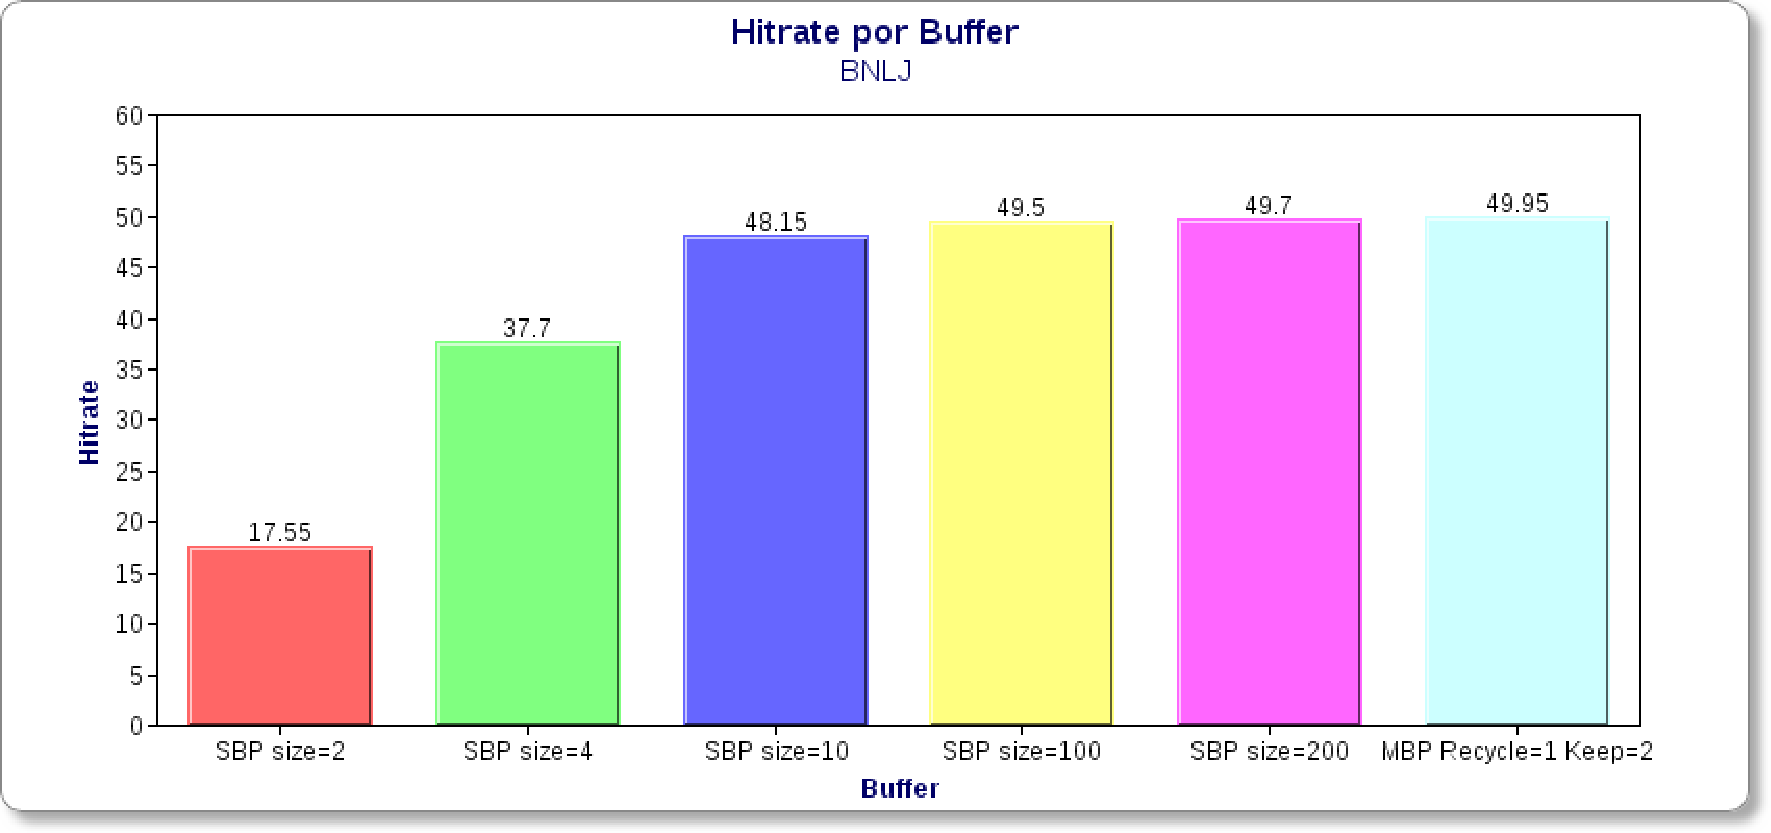
\includegraphics[scale=0.4]{BNLJ.pdf}
    \caption{Gráfico de \textit{hitrate} con respecto a buffer utilizado}
    \label{grafiquito}
\end{figure}

%MANU, SI QUERES HACER GRAFICOS TAN TOP COMO LOS NUESTROS, CLAVATE UN http://www.chartgo.com/. =D =D =D.
%BESITOSSSSSSS Juampi y Juli.

Como se puede observar, con sólamente 3 p\'aginas y una administraci\'on inteligente, la eficiencia
de este mecanismo de m\'ultiples buffers supera a un buffer pool \'unico con tama\~no m\'as de 50 veces mayor.

Otro experimento realizado consistió en simular los accesos a una base de datos realizados
por distintos usuarios. El caso de uso que modelamos ac\'a es realizar accesos a dos tablas,
una chica de 100 p\'aginas y una mucho mas grande, de 10000 p\'aginas. Esto representa de manera
razonablemente fidedigna un \textit{Facebook} simplificado. Se cuenta con una tabla (relativamente) chica de usuarios y 
una tabla gigantesca de interacciones, como pueden ser los \textit{Like} o las publicaciones. 
Se van a acceder de manera muy frecuente a las tablas con la informaci\'on de los usuarios, pero
ocasionalmente a las de interacciones, y de forma esparsa (no secuencial).

Como la tabla de usuarios va a ser accedida frecuentemente, la pondremos en KEEP, mientras
que las de interacciones las vamos a poner en RECYCLE.

Generamos la traza haciendo 200 accesos aleatorios a las 100 p\'aginas de usuario, y de forma
intercalada, generamos 1000 accesos aleatorios a las 10000 p\'aginas de interacciones.

Los resultados obtenidos son:

\begin{table}[H]\centering
    \begin{tabular}{l || c}
    \multicolumn{1}{c ||}{\large{\textbf{Estrategia}}}  & \large{\textbf{Hitrate}} [\%] \\
    \hline
                Multiple Buffer Pools KEEP=20 RECYCLE=1 & 3.08   \\
                Multiple Buffer Pools KEEP=30 RECYCLE=1 & 4.09   \\
                Single Buffer Pools SIZE=21             & 0.66   \\
                Single Buffer Pools SIZE=31             & 0.66   \\
                Single Buffer Pools SIZE=51             & 1.08   \\
                Single Buffer Pools SIZE=101            & 3.01   \\
                \end{tabular}
            \end{table}

\begin{figure}[H]\centering
    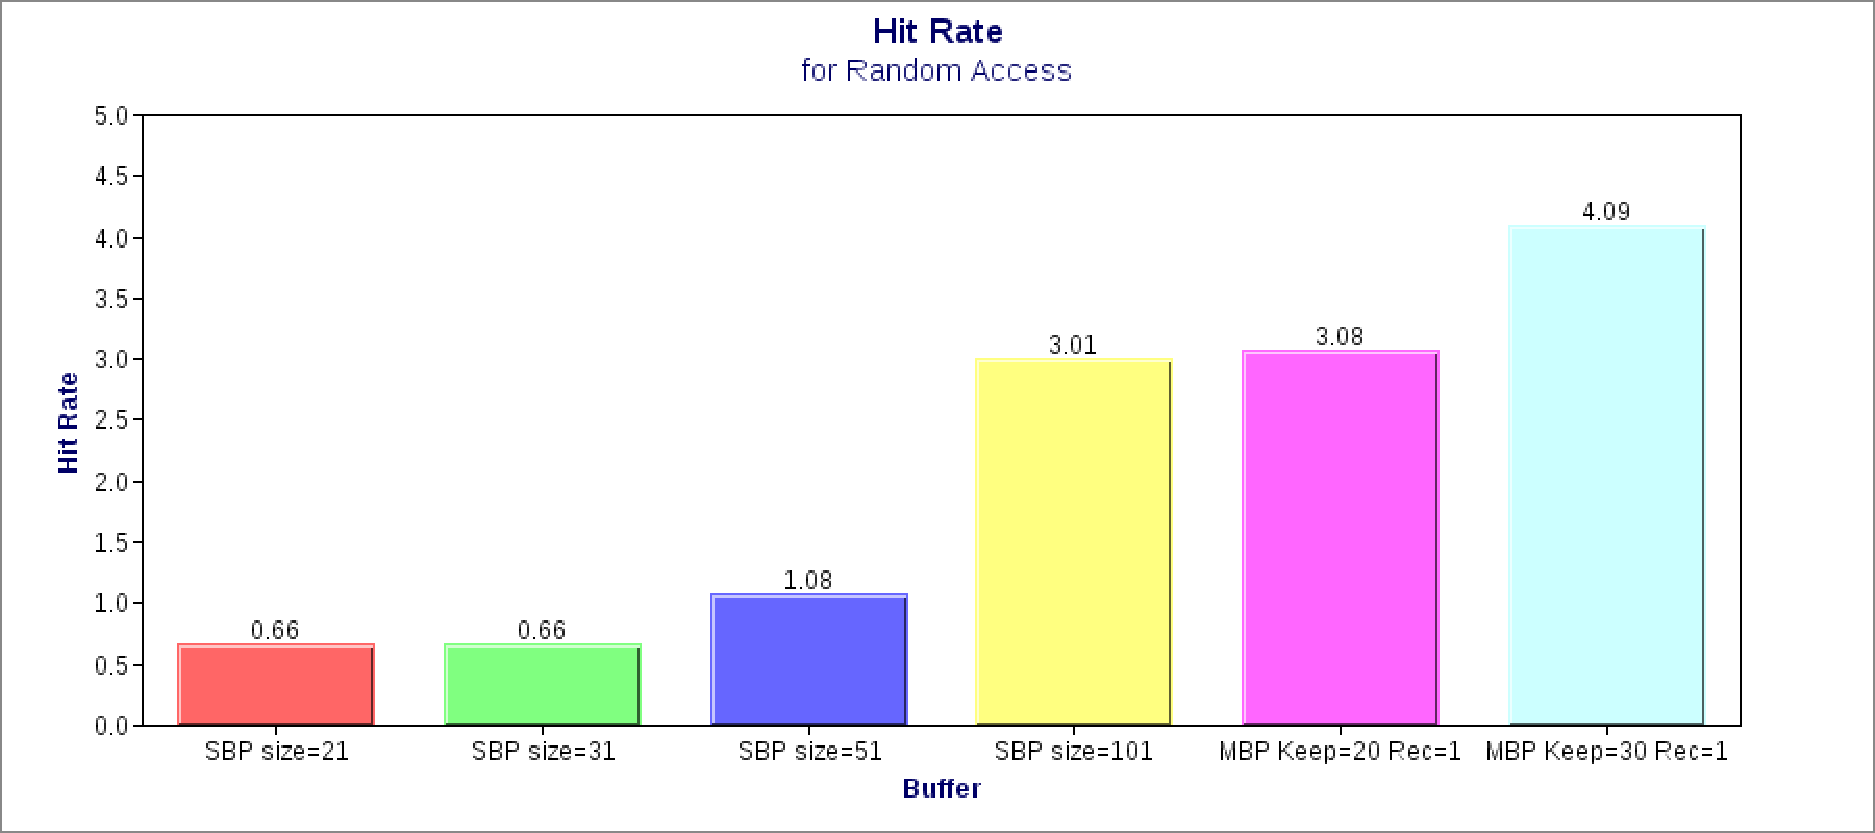
\includegraphics[scale=0.4]{RandomAccess.pdf}
    \caption{Gráfico de \textit{hitrate} para accesos aleatorios con respecto a buffer utilizado}
    \label{grafiquito2}
\end{figure}

Nuevamente, podemos observar que es necesario grandes tama\~nos del single buffer para
poder capturar algo de performance. Hay que tener en cuenta que son accesos aleatorios,
sin patr\'on definido y con que los buffers en memoria puedan capturar un peque\~no 
porcentaje de los accesos m\'as frecuentes basta para traer considerables mejoras al sistema.

También testeamos la eficiencia de un INLJ. Implementamos un generador de traces que simulara un INLJ entre dos tablas.
Este generador toma por cada página de la primera tabla y se le indica cuantas tuplas está guardando en cada página. 
Por cada una de estas tuplas hace una busque en un índice (el cual se le pasa como  parámetro la cantidad de paginas
que tiene y la altura), haciendo $k$ lecturas aleatorios de alguna página, donde $k$ es la altura del árbol. También simula
la búsqueda de páginas en la segunda tabla, se le pasa al generador un número mínimo y máximo de páginas que se 
podrían necesitar buscar en esta segunda página por cada tupla, y se hace R lecturas a de páginas random de la
segunda tabla (donde R es un valor aleatorio en el rango $[min,max]$ especificados como parámetros).

A partir de ahora abreviaremos MBP a \textit{Multiple Buffer Pool} y SBP a \textit{Single Buffer Pool}.

Generamos la traza haciendo un \textit{file scan} de una primer tabla de 100 páginas de tama\~{n}o, por cada una de las paginas
supusimos que tenía 5 tuplas adentro y que cada una de esas tuplas podría encontrar entre 0 y 5 páginas
para leer de la tabla indexada que cuenta con 1000 paginas (con un índice de 5 páginas y de altura 2)

\begin{table}[H]
        \begin{tabular}{l||l}
    \large{\textbf{Estrategia}}                             & \large{\textbf{Hitrate}} [\%] \\
    \hline
                Multiple Buffer Pools KEEP=5 RECYCLE=2		&	47.52	\\
                Multiple Buffer Pools KEEP=50 RECYCLE=2		&	47.52	\\
                Multiple Buffer Pools KEEP=50 RECYCLE=50 	&	49.80	\\
                Single Buffer Pools SIZE=21             	&	31.12	\\
                Single Buffer Pools SIZE=31             	&	40.94	\\
                Single Buffer Pools SIZE=51             	&	44.66	\\
                Single Buffer Pools SIZE=101            	&	45.80	\\
                \end{tabular}
            \end{table}
\begin{figure}[H]\centering
    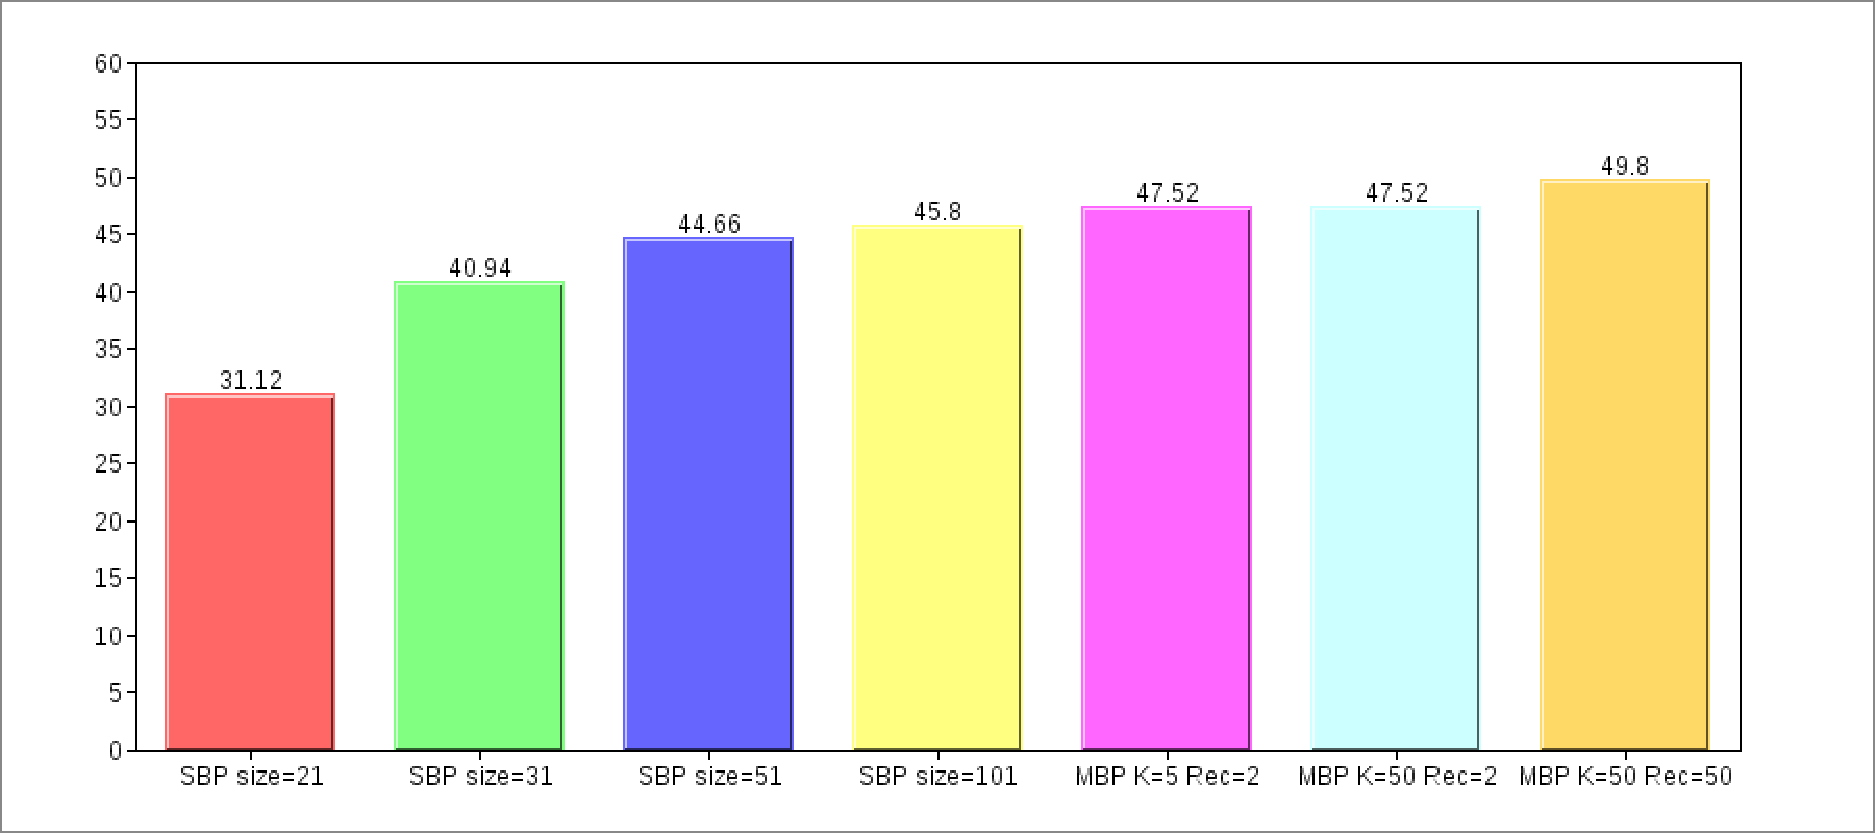
\includegraphics[scale=0.4]{INLJ.pdf}
    \caption{Gráfico de \textit{hitrate} para INLJ con respecto a buffer utilizado}
    \label{grafiquito3}
\end{figure}

Se puede observar que múltiple buffer pool llega rápidamente a su máximo hitrate una vez que keep alcanzada
la cantidad de páginas que cuenta el índice, debido a que tiene los índices en el buffer keep 
y a las dos tablas en recycle. Esto se debe a que para la tabla peque\~{n}a, donde se hace el \textit{scan file}, 
es evidente que no va a dar ni un solo hit por lo que es un claro candidato a recycle, y la tabla con índice,
debido a sus tama\~{n}o, es muy poco probable que vuelva a ser llamada la misma página para que de un hit 
a pesar de tener un tama\~{n}o considerable.

A diferencia del MBP, el SBP comparte las páginas del índice con las otras tablas, por lo que el hitrate
bajo considerablemente, esto puede solucionarse fácilmente manteniendo las páginas del índice en estado
$"REQUEST"$ y liberarlas todas juntas al final, en este caso la performance de SBP sacaría equivalente a la de MBP.

Se puede decir que estos experimentos son conociendo el algoritmo del Or\'aculo,
pero es claramente posible comprobarlo en motores reales. Si se contasen
con estadísiticas de uso de las tablas, sería posible asignarles de manera
din\'amica a que pool van a pertenecer cuando se carguen, e incluso es
posible preveer la performance de las operaciones de acuerdo a que pool
se le asigne, considerando como se la va a emplear. Es decir, no estaría
igual de bien asignar una tabla a \texttt{KEEP} si se la va a usar para \textit{file scan}
una sola vez, que asignar a \texttt{KEEP} una tabla que va a ser usada cientos de veces
en un \texttt{BNLJ}.
